\documentclass{beamer}
\mode<presentation> {
\usetheme{Madrid}
\setbeamertemplate{navigation symbols}{}
}

\usepackage{graphicx} 
\usepackage{booktabs} 
\usepackage[utf8]{inputenc}  
\usepackage[T1]{fontenc}  
\usepackage{geometry}     
\usepackage[francais]{babel} 
\usepackage{eurosym}
\usepackage{verbatim}
\usepackage{ragged2e}
\justifying

%%%%%%%%%%%%%%%%%%%%%%%%%%%%%%%%%%%%%%%%%%%%%%%%%%%%%%%%%%%%%%%%
%% ccBeamer 0.1, 2007-07-02                                   %%
%% Written by Sebastian Pipping <webmaster@hartwork.org>      %%
%% ---------------------------------------------------------- %%
%% Licensed under Creative Commons Attribution-ShareAlike 3.0 %%
%% http://creativecommons.org/licenses/by-sa/3.0/             %%
%%%%%%%%%%%%%%%%%%%%%%%%%%%%%%%%%%%%%%%%%%%%%%%%%%%%%%%%%%%%%%%%


%% Images
\newcommand{\CcImageBy}[1]{%
	
\includegraphics[scale=#1]{creative_commons/cc_by_30.pdf}%
}
\newcommand{\CcImageCc}[1]{%
	
\includegraphics[scale=#1]{creative_commons/cc_cc_30.pdf}%
}
\newcommand{\CcImageDevNations}[1]{%
	
\includegraphics[scale=#1]{creative_commons/cc_dev_nations_30.pdf}%
}
\newcommand{\CcImageNc}[1]{%
	
\includegraphics[scale=#1]{creative_commons/cc_nc_30.pdf}%
}
\newcommand{\CcImageNd}[1]{%
	
\includegraphics[scale=#1]{creative_commons/cc_nd_30.pdf}%
}
\newcommand{\CcImagePd}[1]{%
	
\includegraphics[scale=#1]{creative_commons/cc_pd_30.pdf}%
}
\newcommand{\CcImageSa}[1]{%
	
\includegraphics[scale=#1]{creative_commons/cc_sa_30.pdf}%
}
\newcommand{\CcImageSampling}[1]{%
	
\includegraphics[scale=#1]{creative_commons/cc_sampling_30.pdf}%
}
\newcommand{\CcImageSamplingPlus}[1]{%
	
\includegraphics[scale=#1]{creative_commons/cc_sampling_plus_30.pdf}%
}


%% Groups
\newcommand{\CcGroupBy}[1]{% zoom
	\CcImageBy{#1}%
}
\newcommand{\CcGroupByNc}[2]{% zoom, gap
	\CcImageBy{#1}\hspace*{#2}\CcImageNc{#1}%
}
\newcommand{\CcGroupByNcNd}[2]{% zoom, gap
	\CcImageBy{#1}\hspace*{#2}\CcImageNc{#1}\hspace*{#2}\CcImageNd{#1}%
}
\newcommand{\CcGroupByNcSa}[2]{% zoom, gap
	\CcImageBy{#1}\hspace*{#2}\CcImageNc{#1}\hspace*{#2}\CcImageSa{#1}%
}
\newcommand{\CcGroupByNd}[2]{% zoom, gap
	\CcImageBy{#1}\hspace*{#2}\CcImageNd{#1}%
}
\newcommand{\CcGroupBySa}[2]{% zoom, gap
	\CcImageBy{#1}\hspace*{#2}\CcImageSa{#1}%
}
\newcommand{\CcGroupDevNations}[1]{% zoom
	\CcImageDevNations{#1}%
}
\newcommand{\CcGroupNcSampling}[2]{% zoom, gap
	\CcImageNc{#1}\hspace*{#2}\CcImageSampling{#1}%
}
\newcommand{\CcGroupPd}[1]{% zoom
	\CcImagePd{#1}%
}
\newcommand{\CcGroupSampling}[1]{% zoom
	\CcImageSampling{#1}%
}
\newcommand{\CcGroupSamplingPlus}[1]{% zoom
	\CcImageSamplingPlus{#1}%
}


%% Text
\newcommand{\CcLongnameBy}{Attribution}
\newcommand{\CcLongnameByNc}{Attribution-NonCommercial}
\newcommand{\CcLongnameByNcNd}{Attribution-NoDerivs}
\newcommand{\CcLongnameByNcSa}{Attribution-NonCommercial-ShareAlike}
\newcommand{\CcLongnameByNd}{Attribution-NoDerivs}
\newcommand{\CcLongnameBySa}{Attribution-ShareAlike}

\newcommand{\CcNote}[1]{% longname
	This work is licensed under the \textit{Creative Commons #1 3.0 License}.%
}


\title[Lifehacking]{Lifehacking} 
\author{Genma}

\begin{document}

%% Titlepage
\begin{frame}
	\titlepage
	\vfill
	\begin{center}
		\CcGroupByNcSa{0.83}{0.95ex}\\[2.5ex]
		{\tiny\CcNote{\CcLongnameByNcSa}}
		\vspace*{-2.5ex}
	\end{center}
\end{frame}


%\begin{frame}
%\frametitle{Plan} 
%\tableofcontents
%\end{frame}

%----------------------------------------------------------------------------------------
%	PRESENTATION SLIDES
%----------------------------------------------------------------------------------------


\begin{frame}
\frametitle{
\includegraphics[scale=0.4]{./Genma.jpg} \ \ \  A propos de moi  }
\begin{columns}[c] 

\column{.55\textwidth} 
\textbf{Où me trouver sur Internet?}
\begin{itemize}
\item Le Blog de Genma : http://genma.free.fr
\item Twitter : http://twitter.com/genma
\end{itemize}

\textbf{Mes centres d'intérêts?}
\\ Plein de choses dont:
\begin{itemize}
\item La veille technologique
\item Le chiffrement
\item Le lifehacking
\end{itemize}

\column{.5\textwidth} 
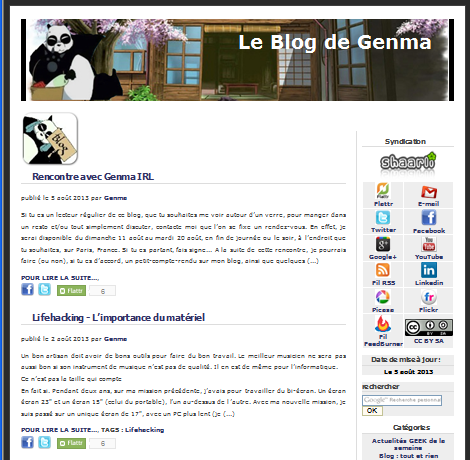
\includegraphics[width=5cm,height=5cm]{blog.png} 

\end{columns}
\end{frame}

%----------------------------------------------------------------------------------------
\begin{frame}
\begin{center}
\Huge{Le lifehacking}
\end{center}
\end{frame}

%----------------------------------------------------------------------------------------
\begin{frame}
\frametitle{Qu'est ce que le Lifehacking?}
\begin{itemize}
\item N'avez vous jamais eu l'impression "de perdre votre temps"?
\item Le lifehacking, c'est chercher à optimiser son temps.
\end{itemize}
$\Rightarrow$  La procrastination n'est pas interdite. 
\\
$\Rightarrow$  Au contraire, elle est planifiable/planifiée.
\end{frame}

%----------------------------------------------------------------------------------------
\begin{frame}
\frametitle{Les méthodes célèbres}
\begin{itemize}
\item Getting Things Done (GTD).
\item Pomodoro.
\item Autres.
\end{itemize}
$\Rightarrow$ Cherchez dans votre moteur de recherche préféré ;-)
\end{frame}

%----------------------------------------------------------------------------------------
\begin{frame}
\frametitle{Mon expérience et mes "outils"}
\begin{itemize}
\item Les pochettes (GTD)
\item Calendrier
\item Todo liste
\item Post-it
\item Les stabylos
\item Google Agenda
\item Un cahier
\item Agendas papier (semainier, mois)
\end{itemize}
\end{frame}

%----------------------------------------------------------------------------------------
\begin{frame}
\frametitle{Et quand on travaille dans l'informatique?}
\begin{itemize}
\item AGIL
\item Les sprints
\item SCRUM etc.
\end{itemize}
$\Rightarrow$ J'ai lu des choses dessus mais j'ai appliqué "ma méthode".
\end{frame}


%----------------------------------------------------------------------------------------
\begin{frame}
\frametitle{En gestion de projet}
\begin{itemize}
\item Le Kanban
\item Les Post-it
\item Les stabylos
\item Le Paper board
\item Le tableau Velleda
\item Les calendriers
\end{itemize}
$\Rightarrow$ Savoir d'où l'on vient, où l'on en est, où l'on va.
\end{frame}

%----------------------------------------------------------------------------------------
\begin{frame}
\frametitle{Le Kanban}
Les différentes colonnes pour de l'Agil / suivi de projet
\begin{itemize}
\item A faire	
\item En cours de développement
\item En cours de test/recette
\item A livrer
\end{itemize}
$\Rightarrow$ On a alors une visibilité sur l'avancement.
\end{frame}

%----------------------------------------------------------------------------------------
\begin{frame}
\frametitle{Le Kanban}
Les différentes colonnes pour de la planification
\begin{itemize}
\item Une colonne est un mois
\item On peut subdiviser en semaine
\end{itemize}
$\Rightarrow$ On a alors une visibilité dans le temps.
\\$\Rightarrow$ Utilité du lifehacking quand on gère plusieurs versions en parallèle.
\end{frame}

%----------------------------------------------------------------------------------------
\begin{frame}
\frametitle{Remarques et conseils}
\begin{itemize}
\item Pour les couleurs (post-it, stylos, stabylos), on peut définir des codes couleurs.
\item Sur les post-it, on met des codes (références), des priorités (P0, P1...)
\item Pour les pochettes, on n'écrit pas directement dessus. On met le titre sur un post-it.
\end{itemize}
\end{frame}

%----------------------------------------------------------------------------------------
\begin{frame}
\frametitle{Conseils}
Trouver sa propre méthode, l'adapter, l'optimiser
\begin{itemize}
\item Des logiciels sur Ordinateurs
\item Tout sur papier
\item Un mix des deux
\end{itemize}
\end{frame}

%----------------------------------------------------------------------------------------
\begin{frame}
\begin{center}
\Huge{Questions et discussion}
\end{center}
\end{frame}


\end{document}